\documentclass[a4paper]{scrreprt}

\usepackage[ngerman]{babel}
\usepackage[utf8]{inputenc}
\usepackage[T1]{fontenc}
\usepackage{lmodern}

\usepackage[german,linesnumbered,algoruled,longend,vlined]{algorithm2e}
\DontPrintSemicolon
\SetArgSty{}
\SetKw{KwOr}{or}
\SetKw{KwAnd}{and}
\SetKw{KwNot}{not}
\setlength{\algomargin}{3ex}

\usepackage[fixlanguage]{mybabelbib}
% \selectlanguage{ngerman}
\setbibliographyfont{title}{}
\setbibliographyfont{jtitle}{}
\setbibliographyfont{btitle}{\emph}
\setbibliographyfont{stitle}{\emph}
\setbibliographyfont{journal}{\emph}

\usepackage{amsmath}
\usepackage{amsfonts}
\usepackage{amssymb}
\usepackage{amsthm}

\usepackage{graphicx}
\usepackage[a4paper,bookmarks,bookmarksnumbered]{hyperref}
\usepackage[font=small,format=hang,labelfont=bf,figurename=Abb.,tablename=Tab.]{caption}
\usepackage{enumerate}

\newtheorem{satz}{Satz}[chapter]
\newtheorem{lemma}[satz]{Lemma}
\newtheorem{beobachtung}[satz]{Beobachtung}
\newtheorem{folgerung}[satz]{Folgerung}
\newtheorem{korollar}[satz]{Korollar}
\theoremstyle{definition}
\newtheorem{definition}[satz]{Definition}
\newenvironment{beweis}{\begin{proof}}{\end{proof}}

\graphicspath{{abbildungen/}}

\begin{document}
%%%%%%%%%%%%%%%%%%%%%%%%%%%%%%%%%%%%%%%%%%%%%%%%%%%%%%%%%%%%%%%%%%%%%%%%%%
%%%%%%%%%%%%% Bitte nur ab hier Änderungen vornehmen %%%%%%%%%%%%%%%%%%%%%

%% hier Titel und Autorennamen eintragen

\subject{Bachelorarbeit} % Geben Sie die Art der Arbeit an
\title{Titel der Arbeit} % Geben Sie hier den Titel Ihrer Arbeit an.
\author{Testvorname Testnachname} % Geben Sie Ihren Namen an. 
\date{Eingereicht am XX. YY 20ZZ} % Geben Sie das Abgabedatum an
\titlehead{Julius-Maximilians-Universität Würzburg\\
Institut für Informatik\\
Lehrstuhl für Informatik I\\
Effiziente Algorithmen und wissensbasierte Systeme}
\publishers{Betreuer:\\
Prof.\ Dr.\ Alexander Wolff\\
Dipl.-Inf.\ Max Mustermann} % Geben Sie den Namen des weiteren Betreuers and
\maketitle


\tableofcontents

\chapter{Kapitel sind ganz einfach}

\section{Abschnitte ebenfalls}

Hier fängt der Text an.

\begin{satz}[Finkscher Hauptsatz] \label{thm:fink}
  Wichtige und grundlegende Sätze lassen sich leicht hervorheben.
\end{satz}

\begin{beweis}
  Der Satz gilt offensichtlich, denn
  \begin{equation*}
    \sum_{i=1}^{n} 1 = n
  \end{equation*}
  Zudem wird der Beweis automatisch mit einem q.e.d.-Symbol beendet.
\end{beweis}

Auf Sätze, wie z.B.\ Satz~\ref{thm:fink}, lässt sich mithilfe des
Befehls \verb+\ref{labelname}+ verweisen, wenn man in der
Satz-Umgebung einen "`Label"' mit \verb+\label{labelname}+ gesetzt
hat.  Genauso können wir auf den nächsten Abschnitt, also
Abschnitt~\ref{sec:leichtigkeit}, verweisen.  Üblicherweise beginnt
man einen Labelnamen mit dem Typ der Umgebung, auf die man verweist,
also z.B.\ \verb+\label{fig:trapez}+ für eine Abbildung (engl.\
\emph{figure}).  Ach ja, zum Hervorheben (engl.\ \emph{emphasize})
eines \emph{neuen Begriffs} verwendet man den Befehl
\verb+\emph{neuer Begriff}+, wenn der neue Begriff zum ersten Mal
verwendet wird.

\section{Zweiter Abschnitt}
\label{sec:leichtigkeit}

\begin{definition}
  Definitionen lassen sich leicht erstellen.
\end{definition}

\begin{figure}[h]
  \centering
  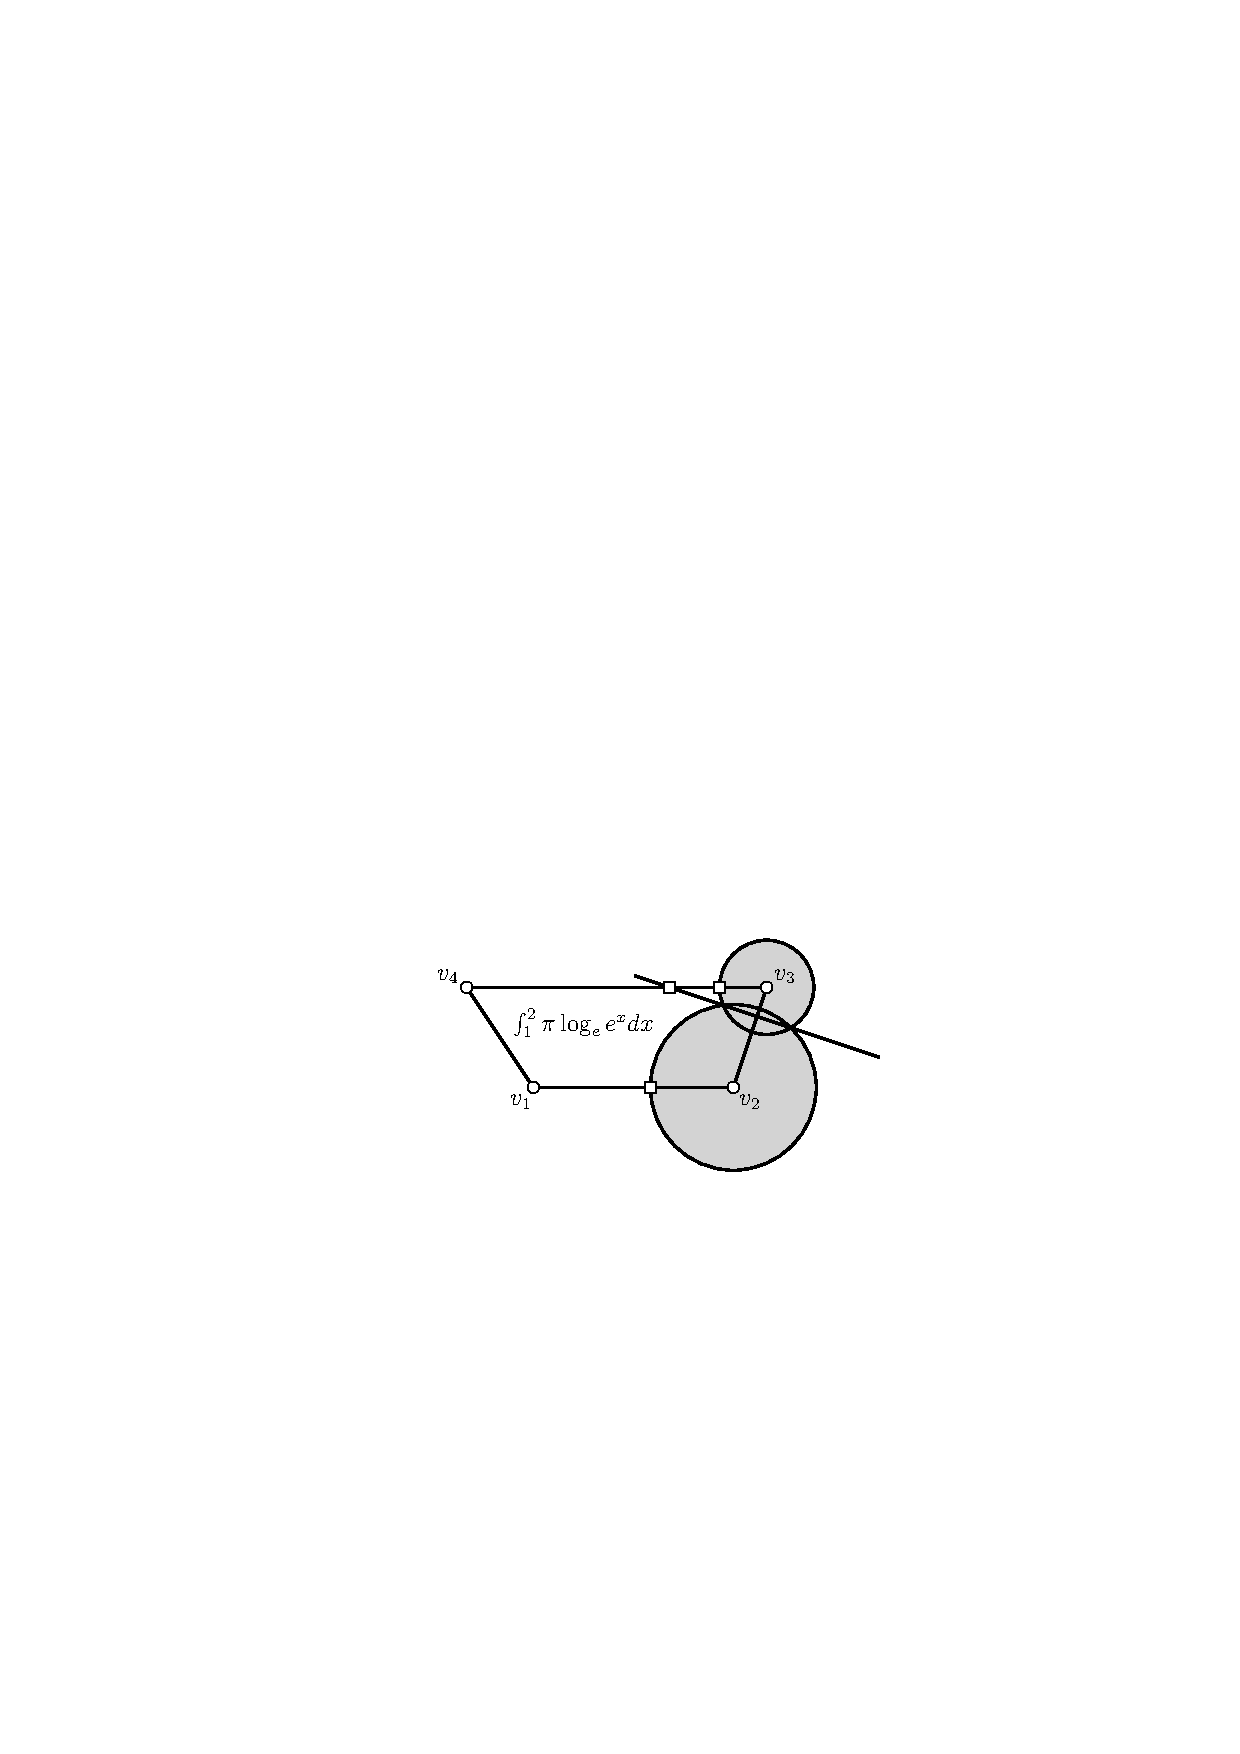
\includegraphics{trapez}
  \caption{Das ist eine Abbildung.}
  \label{fig:trapez}
\end{figure}

Auch Abbildungen, wie z.B.\ Abbildung~\ref{fig:trapez}, sind schnell
eingefügt.  Im Allgemeinen braucht man die Endung der Bilddatei beim
Einbinden mit \verb+\includegraphics+ nicht mit anzugeben.

\subsection{Ein Unterabschnitt}

Zu viele Unterebenen nach Möglichkeit vermeiden. Wir wollen hier nur
zeigen, dass es mit der \verb+algorithm+-Umgebung (aus dem Paket
\verb+algorithm2e.sty+) nicht schwer ist Algorithmen in Pseudocode zu
setzen, siehe Algorithmus~\ref{alg:binsearch}.

\begin{algorithm}[ht]
  \SetKw{True}{true}
  \SetKw{False}{false}
  \caption{BinäreSuche(Feld $A$, ganze Zahl $n$, Element $x$)}
  \label{alg:binsearch}
  \Ein{sortiertes Feld $A$, Länge $n$, gesuchtes Element $x$}
  \Aus{\True genau dann, wenn $x$ in $A$ enthalten ist}
  
  $l = 0$ \;
  $r = n-1$ \;
  
  \While{$l \le r$}{
    $m = \lfloor (l + r)/2 \rfloor$ \;
    \If{$A[m] == x$}{
      \Return \True \;
    }
    \ElseIf{$x < A[m]$}{
      $r = m - 1$ \;
    }
    \Else{
      $l = m + 1$ \;
    }
  }
  \Return \False
\end{algorithm}

Das gleiche geht problemlos auch ohne Zeilennummern, siehe
Algorithmus~\ref{alg:binsearchwithoutlinenumbers}.  Dazu benützt man
einfach in der \verb+algorithm+-Umgebung den Befehl
\verb+\LinesNotNumbered+.

\begin{algorithm}[ht]
  \LinesNotNumbered
  \SetKw{True}{true}
  \SetKw{False}{false}
  \caption{BinäreSucheOhneZeilennum(Feld $A$, ganze Zahl $n$, Element $x$)}
  \label{alg:binsearchwithoutlinenumbers}
  \Ein{sortiertes Feld $A$, Länge $n$, gesuchtes Element $x$}
  \Aus{\True genau dann, wenn $x$ in $A$ enthalten ist}
  
  $l = 0$ \;
  $r = n-1$ \;
  
  \While{$l \le r$}{
    $m = \lfloor (l + r)/2 \rfloor$ \;
    \If{$A[m] == x$}{
      \Return \True \;
    }
    \ElseIf{$x < A[m]$}{
      $r = m - 1$ \;
    }
    \Else{
      $l = m + 1$ \;
    }
  }
  \Return \False
\end{algorithm}

\subsection{Noch ein Unterabschnitt}

Auch Verweise auf ältere Resultate, wie das von Mustermann und
Musterfrau \cite{mustermann+etal-11}, sind ganz einfach.

\bibliographystyle{mybabalpha-fl}
\bibliography{mybib}


\end{document}
